\documentclass[12pt]{article}
\usepackage{graphicx}
\graphicspath{{./}}
\begin{document}

	\title{ELEN3021 (Capstone Project) - Lossless Compression}
	\author{Seale Rapolai - 1098005}
	\maketitle
	
	\section{Introduction}
	\begin{flushleft}
		This report will contains an analysis of the the effects of lossless compression on total transmission time of diffferent file sizes. The compression algorithm used for the analysis below was the Lempel-Ziv-Welch (LZW) algorithm. Furthermore, small files were chosen for this initail analysis. These files contain "Lorem ipsum" (dummy text) text.
	\end{flushleft}
	
	\section{Normal Data Transfer}
	\begin{figure}[ht]
		\begin{center}
			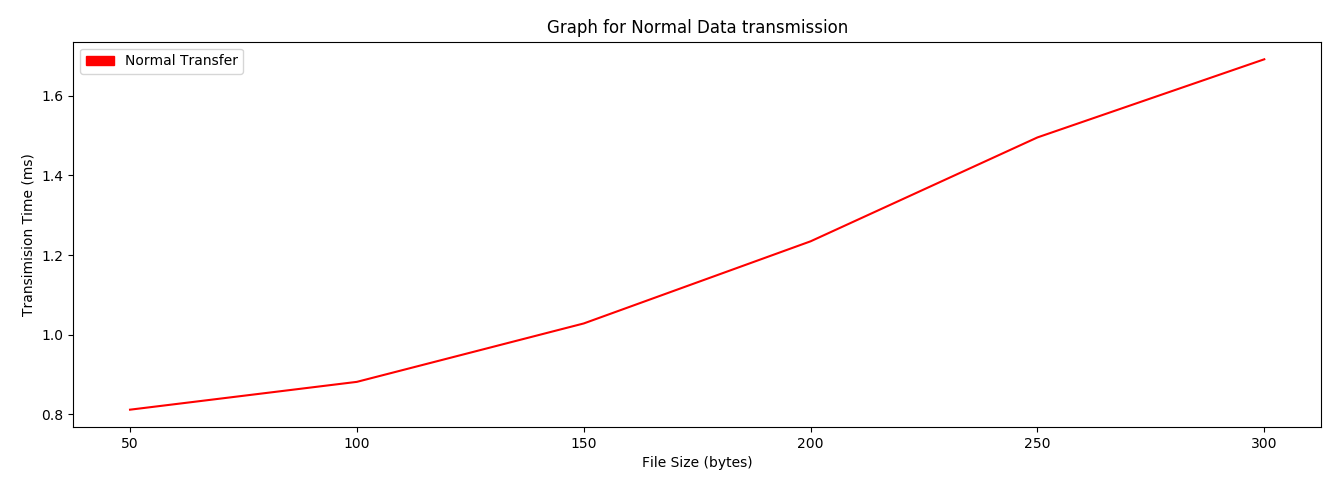
\includegraphics[scale=0.4]{Figure_1.png}
		\end{center}
		\caption{Normal data transfer graph}
	\end{figure}
	
	\begin{flushleft}
		The First test involved measuring the amount of time it took to transfer (copy) a file from one location to the next with compressing or decompressing the file. This tranmission test was performed locally, on the same machine. The file sizes were varied and the transmission time for each file size was recorded and plotted. Figure 1 above summerises the results optained.
	\end{flushleft}
	
	\section{Data Trasnfer with Lossless Compression}
	\begin{figure}[ht]
		\begin{center}
			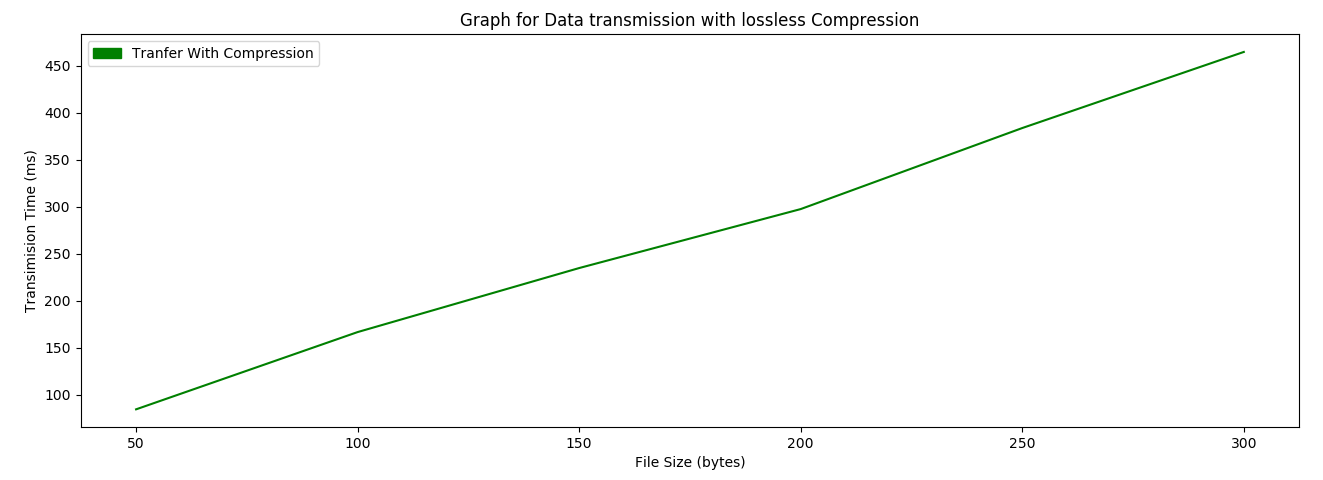
\includegraphics[scale=0.4]{Figure_2.png}
		\end{center}
		\caption{Data transfer with Lossless Compression graph}
	\end{figure}
	
	\begin{flushleft}
		The second test involved measuring the amount of time it took to compress the file, transfer (copy) it from one location to the next and the decompressing it. This transmission test was also performed locally, on the same machine. The file sizes were also varied and the overall time for each file size was recorded and the results were plotted. Figure 2 above summerises these results.
	\end{flushleft}
	
	
	\section{Data Transfer Comparison: Normal VS }
	\begin{figure}[ht]
		\begin{center}
			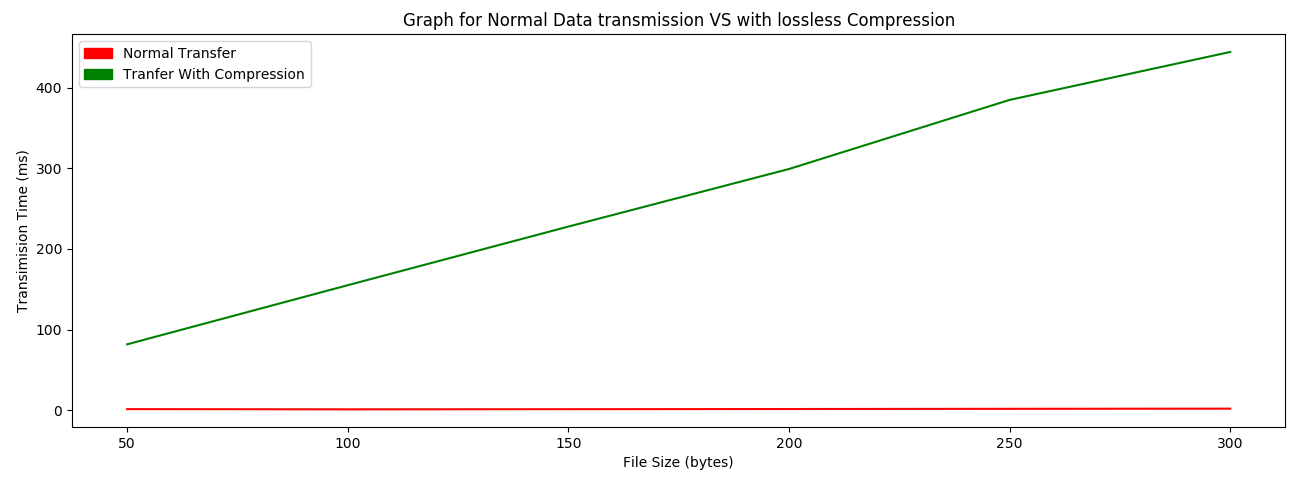
\includegraphics[scale=0.4]{Figure_3.png}
		\end{center}
		\caption{Data transfer with Lossless Compression graph}
	\end{figure}
	
	\begin{flushleft}
		To see if there was an improvement to the data trasnfer the results from both tests were plotted on the same graph and compared. It is clear to that by using lossless compression on the files had a negative effect on the transfer speed of the data.
	\end{flushleft}
	
	\section{Conclusion}
	\begin{flushleft}
		From the analysis conducted above, it may be easy to conclude that lossless compression has a negative effect on data transfer. There is a number of reasons as to why the above results were not as expected. To Further test the effectiveness of this algorithm in data transfer, a more realistic test need to be conducted. This realistic test will include transfering the data over a network to see the effects since transfering data over a network is slower that simply copying the data on the same machine.
		
		Since the aim of this research is test the effects of using lossless compression in data transfer, other a better (prefably faster perfoming) lossless compression algorithms may need to be used. Other alternatives include the Huffman encoding and Shannon fano coding.
	\end{flushleft}
	
\end{document}
